\documentclass[12pt, letterpaper, final]{article}

% All the documents are structured the same way described in a general document
\usepackage[a4paper, left=3.5cm,right=3.5cm,bottom=3.5cm]{geometry}
\usepackage[final]{graphicx}
\graphicspath{{../images/}}
\usepackage{mathrsfs}
\usepackage{newtxtext}
\usepackage{float}
\usepackage{comment}
\usepackage{tikz}
\usetikzlibrary{calc}
\usepackage{eso-pic}
\usepackage[dutch]{babel}
\usepackage{fancyhdr}
\usepackage{multirow}
\usepackage[table]{xcolor}
\usepackage[hidelinks]{hyperref}
\usepackage[toc, acronym, nomain]{glossaries-extra}
\usepackage{attachfile}
\usepackage{array}
\usepackage{xltabular}
\usepackage{hyperref}
\usepackage{float}
\usepackage{url}
\usepackage{xltabular}

% Definieer afkortingen
\newacronym{cnc}{CNC}{Computer Numerical Control}
\newacronym{pid}{PID}{Proportional-Integral-Derivative}
\newacronym{gui}{GUI}{Graphical User Interface}
\newacronym{usb}{USB}{Universal Serial Bus}
\newacronym{AX5140}{AX5140}{Digital Compact Servo Drive welke gemonteerd is in de testkast}

\newacronym{AX5801}{AX5801}{Veiligheidskaart; uitbreiding van de \gls{AX5140}}
\newacronym{AX5701}{AX5701}{Encoder option card; uitbreiding van de \gls{AX5140}}
\newacronym{AX5702}{AX5702}{Encoder option card; zelfde als \gls{AX5701} maar dan met een extra port}

\newacronym{STO}{STO}{Safe Torque Off}
\newacronym{SSI}{SSI}{Synchronous Serial Interface}
\newacronym{PDF}{PDF}{Portable Document Format}
\newacronym{NC}{NC}{Numerical Control}

\newacronym{DFT}{DFT}{Discrete Fourier Transform}
\newacronym{DTFT}{DTFT}{Discrete-time Fourier Transform}
\newacronym{STFT}{STFT}{Short Time Fourier Transform}
\newacronym{FFT}{FFT}{Fast Fourier Transform}

\newacronym{BPFO}{BPFO}{Balls Pass Frequency Outer Race}
\newacronym{BPFI}{BPFI}{Ball Pass Frequency Inner Race}
\newacronym{BSF}{BSF}{Ball Spin Frequency}
\newacronym{FTF}{FTF}{Fundamental Train Frequency}

\newacronym{SS1}{SS1}{Safe Stop 1}

\newacronym{A}{A}{Ampère}
\newacronym{V}{V}{Voltage}
\newacronym{Hz}{Hz}{Hertz}
\newacronym{ms}{ms}{milliseconden}

\newacronym{AC}{AC}{Alternating Current}
\newacronym{EEPROM}{EEPROM}{Erasable Programable Read-Only Memory}
\newacronym{FRAM}{FRAM}{Ferroelectric Random Access Memory}
\newacronym{SoE}{SoE}{\gls{SERCOS} over \gls{EtherCAT}}
\newacronym{SERCOS}{SERCOS}{SErial Real-time COmmunication System}

\newacronym{EtherCAT}{EtherCAT}{Ethernet for Control Automation Technology}
\newacronym{TwinCAT}{TwinCAT}{The Windows Control and Automation Technology}
\newacronym{MQTT}{MQTT}{Message Queuing Telementry Transport}
\newacronym{PLC}{PLC}{Programmable Logic Controller}
\newacronym{ADS}{ADS}{Automation Device Specification}
\newacronym{IDN}{IDN}{Identification Number}
\newacronym{WPF}{WPF}{Windows Presentation Foundation}
\newacronym{POC}{POC}{Proof Of Concept}
\newacronym{dB}{dB}{Decibel}

\newacronym{MCSA}{MCSA}{Motor Current Signature Analysis}
\newacronym{RMS}{RMS}{Root Mean Squared}

\newacronym{HMI}{HMI}{Human Machine Interface}

\newacronym{CPK}{CPK}{Capability Index}
\newacronym{CP}{CP}{Capability of the process}

\newacronym{USL}{USL}{Upper Specification Limit}
\newacronym{LSL}{LSL}{Lower Specification Limit}

\newacronym{SRD}{SRD}{System Requirement Document}

\newacronym{CTQ}{CTQ}{Critital To Quality}

\makeglossaries

\usepackage{chngcntr}
\numberwithin{figure}{section}
\numberwithin{table}{section}

% Mooi hoekje links bovenin net als in de Voortman template
\newcounter{pagecount}
\AtBeginShipout{%
	\stepcounter{pagecount} % Tel de pagina's
	\ifnum\value{pagecount}>1 % Pas toe vanaf pagina 2
	\AtBeginShipoutUpperLeft{%
		\begin{tikzpicture}[remember picture, overlay]
			\fill[customred] (current page.north west) ++(3.0cm,0) -- (current page.north west) -- ++(0,-6.5cm) -- cycle;
		\end{tikzpicture}
	}
	\fi
}

\pagestyle{fancy}

\fancyhf{}

\definecolor{customred}{HTML}{D78C91}

\newenvironment{myfont}{\fontfamily{phv}\selectfont}{\par}

\fancyhead[L]{\textbf{Afstudeerstage}}
\fancyhead[C]{}
\fancyhead[R]{\today}

% Voettekst-instellingen
\fancyfoot[L]{Auteur: Florent Kegler}
\fancyfoot[C]{Pagina \thepage}
\fancyfoot[R]{
\includegraphics[width=4cm]{VoortmanLogo}}

% maak de tabel ietsje groter want de standaard is soms beetje smal
\setlength{\arrayrulewidth}{0.5mm}
\setlength{\tabcolsep}{18pt}
\renewcommand{\arraystretch}{1.5}

% Makkelijk commando om eisen in te voegen met xltabular
\newcommand{\eistabel}[6]{
	\begin{xltabular}{\linewidth}{|p{0.15\linewidth}|p{0.5\linewidth}|p{0.2\linewidth}|}
		\caption{#1 #2}\\
		\hline
		\textbf{#1} & \textbf{#2} & \textbf{#3} \\
		\hline
		\endfirsthead
		\hline
		\textbf{#1} & \textbf{#2} & \textbf{#3} \\
		\hline
		\endhead
		\hline
		\endfoot
		\hline
		\endlastfoot
		\textbf{Stelling} & \multicolumn{2}{p{0.7\linewidth}|}{#4}\\
		\hline
		\textbf{Meetmethode} & \multicolumn{2}{p{0.7\linewidth}|}{#5} \\
		\hline
		\textbf{Opmerking} & \multicolumn{2}{p{0.7\linewidth}|}{#6} \\
		\hline
	\end{xltabular}
}

\begin{document}
	\newcommand{\thesisAuthor}{Florent Kegler \newline 514277}
\newcommand{\thesisTitle}{Functioneel Ontwerp}
\newcommand{\thesisSubTitle}{Ontwikkeling van een Universele Parameter set voor Spindletesten}
\newcommand{\thesisDegree}{Afstudeerstage}
\newcommand{\university}{Saxion University of Applied Sciences}
\newcommand{\credits}{30 ECTS}
\newcommand{\faculty}{Faculteit Engineering}
\newcommand{\thesisPlaceDate}{\today}
\newcommand{\company}{Voortman Steel Machinery}

% Only create some information in the form of commands. The rest is always the same in the general titelpage
\begin{titlepage}
	\input{../GeneralTeX/GeneralTitelpage}
\end{titlepage}
	\tableofcontents
\newpage
\listoftables
\newpage
\listoffigures
\newpage
\printglossary[type=\acronymtype,style=long,title=Afkortingen en Acroniemen,label=tab:Afkortingen]
	\section{Doelstelling}

Op het moment zit er een Beckhoff \gls{AX5140} servo drive in de testkast gebouwd
voor het aansturen van de motoren. De parameters die in deze drive zitten kunnen
momenteel alleen de servomotor HQL100X aansturen. Andere motoren kunnen
niet worden aangestuurd met deze parameters omdat deze motoren bijvoorbeeld
een andere encoder hebben, andere \gls{pid}-instellingen of de motor werkt simpelweg
volgens een ander principe (asynchrone of synchrone servo). De \gls{AX5140} heeft
meer dan 400 parameters de meeste hiervan kunnen worden aangepast. Naast deze
parameters zijn er ook nog parameters instelbaar aan de \gls{PLC} kant in de zogehete
\gls{NC}-task die verantwoordelijk is voor het aansturen van de drive.

\vspace{0.5cm}

Ook is het testprotocol van Voortman op de spindels niet erg geavanceerd zo
worden motoren alleen aangestuurd naar een bepaald tourental voor een bepaald
aantal seconden waarbij er gelet wordt of de motor niet te veel trilt en of deze niet
te warm wordt. Zij kwantificeren deze waardes niet het is daarom erg lastig om
aantoonbaar de motor te beoordelen op zijn prestaties.

\vspace{0.5cm}

De wens is daarom vanuit Voortman om uit te zoeken welke parameters relevant
zijn voor wanneer er een motor gewisseld wordt en welke waardes dit moeten zijn
voor de motoren die zij willen gaan testen. Met daarbij een programma die ervoor
kan zorgen dat deze parameters eenvoudig naar de drive kunnen worden geschreven.
Daarnaast zou het mooi zijn als er uitgezochtwordtwatVoortman wil gaan testen aan
de motoren en wat hiervoor eventueel voor nodig is zoals een trilling sensor die de
trillingen van de spindel kan meten zodat de testen op de motoren gekwantificeerd en
gedocumenteerd kunnen worden in plaats van de huidige manier van testen waarbij
er niks aan de motor gemeten wordt.

\begin{figure}[H]
	\centering
	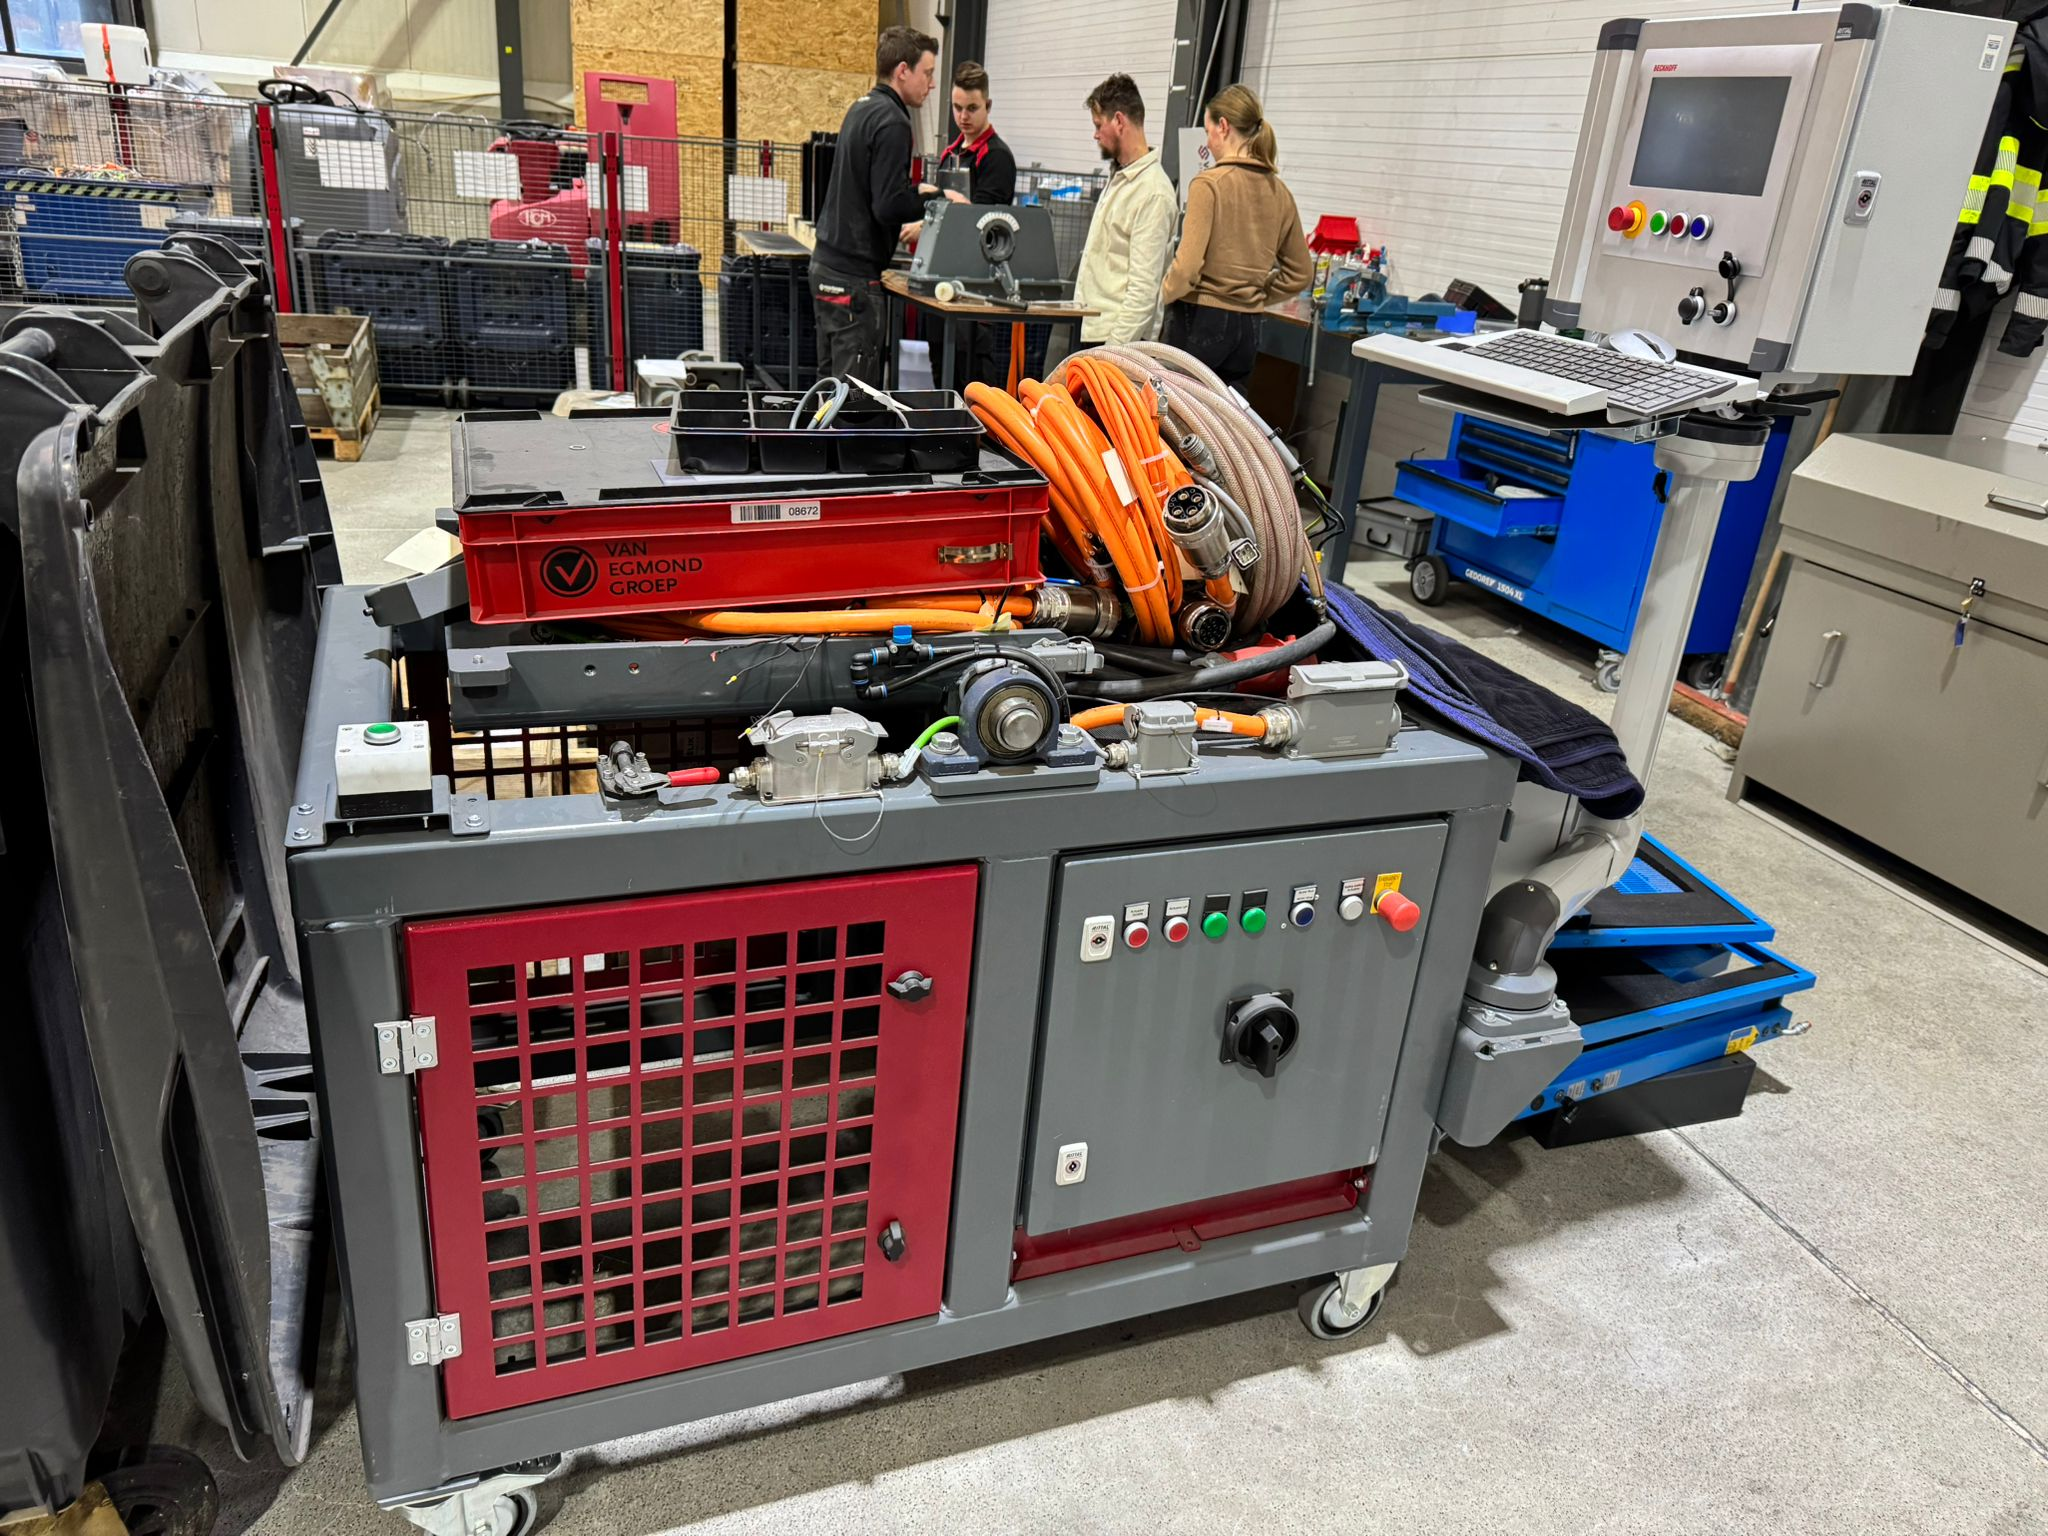
\includegraphics[width=0.7\linewidth]{TestKast}
	\label{fig:Testkast}
	\caption{De testkast in kwestie}
\end{figure}
	\section{Gebruikers Beschrijving}

\subsection{Belanghebbenden}
In deze sectie van het SRD worden de belanghebbende van de opdracht geïdentificeerd. Er zal ook worden beschreven wat de behoeften zijn van de belanghebbenden, die uiteindelijk zullen worden overwogen in het ontwerpproces.

\textbf{Belanghebbenden:}

\begin{itemize}
	\item \textbf{Customer Service (Hoofdgebruiker van de testkast)}
	\begin{itemize}
		\item De customer serviceafdeling zal de testkast gaan gebruiken om teruggestuurde spindels te testen en te analyseren. De behoeften van deze afdeling zullen zijn:
		\begin{enumerate}
			\item Een gebruiksvriendelijke interface om verschillende spindels te testen op de testkast.
			
			\item De testresultaten moeten betrouwbaar zijn en reproduceerbaar.
			
			\item Log bestanden en testrapporten om analyses uit te voeren.
			
			\item Test criteria waar de motoren aan moeten voldoen zodat ze als goed of slecht kunnen worden bestempeld.
			
			\item Meerdere soorten motoren moeten werken op de testkast.
			
			\item Documentatie om de kast te bedienen.
		\end{enumerate}
	\end{itemize}
	
	\item \textbf{Operators (Dagelijkse gebruikers van de testkast)}
	\begin{itemize}
		\item De operators van de testkast zijn de mensen die de kast daadwerkelijk gaan gebruiken. Hun behoeften kunnen zijn:
		\begin{enumerate}
			\item Een gemakkelijke manier om de testparameters voor een specifieke spindel te selecteren.
			
			\item Een veilig systeem wat de risico’s minimaliseert tijdens het testen van de spindels.
			
			\item Een testproces wat niet te veel tijd kost.
			
			\item Duidelijke feedback van de testkast als eventuele problemen zich voor doen. (Foutmeldingen of waarschuwingen)
			
			\item Eventueel vertaalde tekst op het scherm in andere talen.
		\end{enumerate}
	\end{itemize}
	
	\item \textbf{Onderhoudsdienst}
	\begin{itemize}
		\item De onderhoudsdienst is verantwoordelijk voor het onderhoud van de testkast en eventuele uitbreiding van de kast. De behoeften van deze groep is:
		\begin{enumerate}
			\item Goede documentatie van de code.
			
			\item Inzicht in de parameters en instellingen van de testkast.
			
			\item Goed documentatie van de hardware.
		\end{enumerate}
	\end{itemize}
	
	\item \textbf{R\&D Engineering Team}
	\begin{itemize}
		\item Wanneer Voortman besluit nieuwe machines te ontwikkelen met mogelijk nieuwe type spindels kan de testkast ook nuttig zijn voor de R\&D. Zij zouden de volgende dingen willen:
		\begin{enumerate}
			\item Makkelijk nieuwe testscenario’s kunnen instellen voor de nieuwe motoren.
			
			\item Overzicht over de prestaties van de spindel.
		\end{enumerate}
	\end{itemize}
	
	\item \textbf{Klanten van Voortman}
	\begin{itemize}
		\item Klanten die de gereviseerde motor uiteindelijk kopen kunnen ook baat hebben bij de testkast zij zouden de volgende dingen willen hebben:
		\begin{enumerate}
			\item Een testrapport waarin te zien is dat de gekochte gereviseerde spindel correct werkt naar behoren.
		\end{enumerate}
	\end{itemize}
\end{itemize}

\newpage

\subsection{Gebruikersscenario(s)}

In deze sectie worden alle verschillende gebruikersscenario’s geschetst om de interactie die de gebruiker heeft met het systeem te visualiseren. De volgende stappen moeten doorlopen worden om de spindel juist aan te sluiten en te testen op de testkast.

\begin{figure}[H]
	\centering
	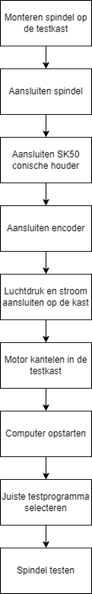
\includegraphics[width=0.18\linewidth]{Gebruikersscenario}
	\label{fig:Gebruikersscenario}
	\caption{Gebruikersscenario spindel bedienen}
\end{figure}

\newpage

\begin{itemize}
	\item \textbf{Monteren spindel op de testkast} houdt in dat de spindel met tenminste twee bouten wordt vastgedraaid op de testkast zodat deze niet meer kan bewegen.
	
	\item \textbf{Aansluiten spindel} betekent dat de drive wordt aangesloten op de spindel.
	
	\item \textbf{Aansluiten SK50 conische houder} betekent dat de luchtcilinders worden aangesloten op de testkast en dat de sensor die checkt of de houder goed gesloten is aangesloten wordt.
	
	\item \textbf{Aansluiten encoder} houdt in dat de encoder wordt aangesloten op de motordrive.
	
	\item \textbf{Luchtdruk en stroom aansluiten op de testkast} houdt in dat de testkast aangesloten wordt op het lichtnet en op de luchtdruk.
	
	\item \textbf{Motor kantelen in de testkast} houdt in dat de spindel wordt gekanteld doormiddel van een Linak actuator binnen in de testkast dit zorgt ervoor dat het draaiende gedeelte van de spindel niet of moeilijker bereikbaar wordt voor de gebruiker dit waarborgt de veiligheid van de gebruiker.
	
	\item \textbf{Computer opstarten} nu alles gereed is kan de computer opgestart worden het testprogramma zou automatisch moeten verschijnen.
	
	\item \textbf{Juist programma kiezen} wanneer de computer is opgestart kan er een testprogramma worden gekozen de juiste parameters worden dan in de drive geladen en de spindel is klaar om getest te worden.
	
	\item \textbf{Spindel testen} de spindel kan nu getest worden.
\end{itemize}

\newpage

\subsection{Voorbeeld eis}

In deze sectie is een kort voorbeeld gemaakt over hoe de eisen in elkaar zitten. Dit is te zien in onderstaande tabel.

\eistabel{Uniek ID}{Titel}{Prioriteit}{Eis van de stelling}{Meetmethode}{Eventuele opmerkingen}

De bovenste rij van de tabel geeft de volgende dingen weer:

\begin{itemize}
	\item \textbf{Uniek ID}
	\begin{itemize}
		\item Elke eis heeft zijn eigen unieke ID zodat hier later naar verwezen kan worden.
	\end{itemize}
	
	\item \textbf{Titel}
	\begin{itemize}
		\item Elke eis heeft zijn eigen titel die kort de eis beschrijft.
	\end{itemize}
	
	\item \textbf{Prioriteit}
	\begin{itemize}
		\item Niet elke eis is urgent en daarom heeft elke eis zijn eigen prioriteit. Er zijn vier prioriteiten: URGENT, HOOG, GEMIDDELD en LAAG.
	\end{itemize}
\end{itemize}

De rest van de tabel omvat het volgende:

\begin{itemize}
	\item \textbf{Stelling}
	\begin{itemize}
		\item Een duidelijke en beknopte beschrijving van de eis.
	\end{itemize}
	
	\item \textbf{Meetmethode}
	\begin{itemize}
		\item Een methode hoe de eis gevalideerd gaat worden in de testfase van het project.
	\end{itemize}
	
	\item \textbf{Opmerking}
	\begin{itemize}
		\item Om onduidelijkheden te verhelpen kan er nog een aanvullende opmerking worden toegevoegd in deze rij.
	\end{itemize}
\end{itemize}

\subsection{Functionele eisen}

\eistabel{FR-001}{Geautomatiseerd testen}{URGENT}{De testkast moet in staat zijn om geautomatiseerd te kunnen testen. Dit houdt in dat er testen gemaakt moeten kunnen worden die vervolgens uitgevoerd kunnen worden op de testkast.}{De eis is behaald wanneer een operator, die los staat van dit project, op de testkast een test kan maken met het instructieboekje en deze ook kan afspelen op de testkast. Deze testkast moet deze test dan automatisch afspelen.}{De operator moet tenminste de keuze hebben uit welk toerental, hoe snel de spindel deze moet bereiken en voor hoelang de spindel moet draaien in dit toerental.}
\eistabel{FR-002}{Testrapport}{GEMIDDELD}{De testkast moet in staat zijn om na afloop van de test een rapport te maken waarin de resultaten van de test staan.}{De eis is behaald wanneer het programma op de testkast een testrapport maakt na afloop van de test. De door de operator gekozen parameters moeten tijdens de test gemonitord worden en weergegeven worden in het rapport. Ook de hoeveelheid samples per seconde moet door de operator gekozen kunnen worden.}{}
\eistabel{FR-003}{Spindel validatie}{LAAG}{Na afloop van de test moet de testkast doormiddel van een statistische analyse van de opgenomen parameters aan kunnen geven of dit binnen de toegestane toleranties en specificaties valt, en of de spindel als ‘goed’ of ‘afgekeurd’ geclassificeerd moet worden.}{De eis is behaald wanneer de testkast spindels kan keuren op basis van tenminste het stroomverbruik deze mag niet significant afwijken van nieuwe spindels met een betrouwbaarheidsinterval van 95\%. De controlegroep moet hiervoor normaal verdeeld zijn met ideaal >30 observaties van nieuwe correct werkende spindels op verschillende toerentallen.}{}
\eistabel{FR-004}{Real time grafieken}{HOOG}{Tijdens de test moeten er op het scherm grafieken komen met real-time data van de spindel. Welke data er op het scherm moet komen moet kunnen worden gekozen door de gebruiker.}{De eis is behaald wanneer de gebruiker een willekeurige parameter kan kiezen en deze kan monitoren op de \gls{gui} tijdens de test. Ook de hoeveelheid samples per seconde moet gekozen kunnen worden door de gebruiker.}{}
\eistabel{FR-005}{Op afstand testen}{GEMIDDELD}{Wanneer de testkast bezig is moet de gebruiker op afstand de testgegevens kunnen bekijken via bijvoorbeeld het \gls{MQTT}-protocol op grafana.}{De eis is behaald wanneer de gebruiker tenminste het stroomverbruik en hoelang het testen nog duurt kan monitoren vanaf een andere laptop die niet is aangesloten op de testkast.}{}
\eistabel{FR-006}{Automatisch parameters inladen}{URGENT}{De testkast moet geautomatiseerd andere parameters in kunnen laden van andere motoren.}{De eis is behaald op het moment dat er een andere motor wordt aangesloten dat de gebruiker slechts door de motor te selecteren in de \gls{gui} de parameters kan inladen in de drive die passen bij die motor.}{}
\eistabel{FR-007}{Handmatig testen}{URGENT}{De gebruiker moet de spindels handmatig kunnen aansturen met de \gls{gui} op de testkast. }{Deze eis is behaald wanneer de gebruiker handmatig de motor kan aansturen met de \gls{gui} op de testkast.}{Het aansturen kan bijvoorbeeld met een slider.}
\eistabel{FR-008}{TwinSAFE geconfigureerd}{GEMIDDELD}{De veiligheidskritieke onderdelen in de testkast zoals de deurschakelaars maar ook de motordrive moeten worden geconfigureerd in een TwinSAFE project zodat de veiligheid van de gebruiker te allen tijde kan worden gewaarborgd.}{Deze eis is behaald wanneer de motor automatisch en gecontroleerd wordt afgeremd met een TwinSAFE project zodra één van de volgende veiligheidsvoorwaarden worden geactiveerd:
\begin{itemize}
	\item Deurbeveiliging: op het moment dat er een deur op de testkast geopend wordt.
	\item Noodstop: wanneer de noodstop wordt ingedrukt.
	\item Wanneer veiligheidslimieten worden overschreden: Bijvoorbeeld een te hoge stroomafwijking.
\end{itemize} De motor moet zo snel mogelijk afremmen. Omdat dit sterk afhankelijk is van welk type motor en welke massatraagheid de spindel heeft en mogelijk nog de tool die hierin zit kan hier geen vaste waarde aan gehangen worden.}{Momenteel is deze veiligheid al wel ingebouwd in de testkast echter is dit niet gedaan met TwinSAFE maar gewoon geprogrammeerd in een \gls{TwinCAT} \gls{PLC} project. }
\eistabel{FR-009}{Servo Motoren}{URGENT}{Tenminste de volgende motoren moeten kunnen worden aangestuurd door de AX5140 motordrive:
\begin{itemize}
	\item MAD100D-0250-SA-C0-AK0-35-N3 (V623) Async servo motor
	\item MAD130C-0150-SA-S2-AP0-05-N1 (V633, V310 nieuw) Async servo motor
	\item HQL100X (V310 oud) Async servo motor
	\item MSK101D-0450-NN-M1-AP0-NNNN (V505-250T, V320, V330C, V320C en V600) Sync servo motor
	\item MS2N10-D0BNN-AMVK0-NNNNN-NN (V630 nieuw)  Sync servo motor
	\end{itemize}}{Deze eis is behaald wanneer bovenstaande motoren aangestuurd kunnen worden vanaf de drive de motoren moeten hierbij draaien.}{Het aansturen kan bijvoorbeeld met een slider.}
\eistabel{FR-010}{FFT-analyse}{LAAG}{De Testkast moet een Fast Fourier Analysis (\gls{FFT}) kunnen uitvoeren op de gemeten trilling gegevens om frequentiespectra te genereren.}{De eis is behaald wanneer de testkast de spindel die getest wordt kan vergelijken met een aantal juist werkende spindels op basis van de trillingen van de motor en ook kan aangeven waar de verschillen zitten om zo mogelijke problemen aan te kunnen duiden.
	
	\vspace{0.5cm}
Meet eerst de trillingen van de motor bij 20\%, 50\% en 80\% van de maximum snelheid.

Voer de fourier transformatie uit op de samples. De formules hiervan zijn te vinden in bijlage \ref{sec:FourierTransform}.

De Referentie $X_k$ is betrouwbaarder wanneer hier een gemiddelde van wordt genomen met ideaal meer dan 30 samples maar aangezien dit veel tijd kan kosten is het ook al waardevol om dit met minder spindels te doen. Dit gemiddelde kan berekend worden met de volgende formule:

\begin{equation}
	\bar{X}_k=\frac{1}{M}\sum_{i=1}^{M}X_{i,k}
\end{equation}

$M$ is hier het aantal referentie metingen (aantal juiste spindels)

Vervolgens om aan te geven hoeveel afwijking er mag zijn bij goede spindels kan de standaarddeviatie per frequentie worden berekend met de volgende vergelijking:

\begin{equation}
	\sigma_k=\sqrt{\frac{1}{M}\sum_{i=1}^{M}(X_{i,k}-\bar{X}_k)^2}
\end{equation}

De testkast moet vervolgens de verschilspectra laten zien door een soort heat map te laten zien waar de grootste afwijkingen zitten dit kan makkelijk met de volgende formule:

\begin{equation}
	\Delta X_k=\frac{|X_{gereviseerd,k} - \bar{X}_k|}{\sigma_k}
\end{equation}

Dit geeft de afwijking in termen van de standaarddeviatie per frequentie. Als $\Delta X_k$ nu groter is dan 2 betekend dit dat het meer dan 2x de standaarddeviatie is. Dit kan betekenen dat de trillingen te veel afwijken bij een bepaalde frequentie van een normale spindel bij een bepaalde frequentie wat kan wijzen op problemen \cite{web:FLUKE}. 

}{Mochten de frequenties nou erg afwijken in de tijd kan er ook mogelijk een spectrogram gemaakt worden in de tijd of eventueel tegen de motorsnelheid in plaats van de tijd.
\gls{STFT} (Short Time Fourier Transform) \cite{web:STFT} .
Door de PLC cycle snelheid zou de sampling frequentie niet zo hoog kunnen zijn dit zal voor de test betekenen dat hogere frequenties niet kunnen worden geanalyseerd omdat hier aliasing zal optreden.
}
\eistabel{FR-011}{\gls{MCSA} (Motor Current Signature Analysis)}{MEDIUM}{De testkast moet een \gls{FFT} kunnen uitvoeren op de meet gegevens van alle fasen van de motor als functie van de tijd om wikkelfouten, lager schade of speling te analyseren.}{De eis is behaald als de testkast de spindel die getest wordt kan vergelijken met een aantal juist werkende spindels op basis van de variatie in stroom per fase van de motor. De methode hiervan is grotendeels hetzelfde als FR-010 en zal daarom niet uitgebreid uitgelegd worden hieronder.

\vspace{0.5cm}

Meet de stroom per fase bij de in FR-010 beschreven snelheden en pas de \gls{DFT} hierop toe om de volgende data reeksen te krijgen: $I_U\left(\mathcal{F}\right)$, $I_V\left(\mathcal{F}\right)$ en  $I_W\left(\mathcal{F}\right)$ bij elke snelheid.

\vspace{0.5cm}

Gebruik net als bij de trillingen meerdere juist werkende motoren om een gemiddeld spectrum te krijgen met daarbij de standaarddeviatie per frequentie.

\vspace{0.5cm}

${\bar{I}}_U\left(\mathcal{F}\right), {\bar{I}}_V\left(\mathcal{F}\right)$ en ${\bar{I}}_W\left(\mathcal{F}\right)$

\vspace{0.5cm}

${\sigma I}_U\left(\mathcal{F}\right), {\sigma I}_V\left(\mathcal{F}\right)$ en $\sigma I_W\left(\mathcal{F}\right)$

\vspace{0.5cm}

Er moeten vervolgens drie heatmaps gemaakt worden voor elke fase één van de gestandaardiseerde afwijking per frequentie met de volgende formules:

\begin{equation}
	\Delta I_U\left(\mathcal{F}\right)=\frac{\left|{I_U\left(\mathcal{F}\right)}_{gereviseerd}-{\bar{I}}_U\left(\mathcal{F}\right)\right|}{{\sigma I}_U\left(\mathcal{F}\right)}
\end{equation}

\begin{equation}
	\Delta I_V\left(\mathcal{F}\right)=\frac{\left|{I_V\left(\mathcal{F}\right)}_{gereviseerd}-{\bar{I}}_V\left(\mathcal{F}\right)\right|}{{\sigma I}_V\left(\mathcal{F}\right)}
\end{equation}

\begin{equation}
	\Delta I_W\left(\mathcal{F}\right)=\frac{\left|{I_W\left(\mathcal{F}\right)}_{gereviseerd}-{\bar{I}}_W\left(\mathcal{F}\right)\right|}{{\sigma I}_W\left(\mathcal{F}\right)}
\end{equation}

Wanneer een waarde hoger is dan 2 op een bepaald punt kan dit wijzen op een significante afwijking ten opzichte van de juiste spindels. Afwijkingen in de frequentie van de stroom kunnen duiden op asymmetrie, magneetschade (bij synchrone motoren), slechte wikkelingen of een ongelijke belasting. 

}{Mochten de frequenties nou erg afwijken in de tijd kan er ook mogelijk een spectrogram gemaakt worden in de tijd of eventueel tegen de motorsnelheid in plaats van de tijd. (\gls{STFT}) \cite{web:STFT}
Door de \gls{SoE} communicatiesnelheid en de \gls{PLC} cyclus snelheid zou de sampling frequentie niet zo hoog kunnen zijn dit zal voor de test betekenen dat hogere frequenties niet kunnen worden geanalyseerd omdat hier aliasing zal optreden.
}
\eistabel{FR-012}{\gls{RMS} (Root Mean Squared) of the motor vibration}{MEDIUM}{De testkast moet aan kunnen geven of de spindel gemiddeld gezien significant meer trilt dan de referentie spindel.}{De eis is behaald wanneer de testkast de gemeten trillingen vergelijkt met de referentie spindel metingen. Dit kan worden berekend op de volgende manier:
	
	Om te weten of de spindel meer of minder trilt kan worden gebaseerd op de RMS-waarde van de sample de formule hiervoor is als volgt:
	
	\begin{equation}
		X_{RMS}=\sqrt{\frac{1}{n}\sum_{i=0}^{n-1}X_i^2}
	\end{equation}
	
	
	Deze waarde van de gereviseerde spindel mag niet te veel afwijken van de gemiddelde waarde van de referentiegroep (juist werkende spindels) +- 2x de standaarddeviatie hiervan. Waarbij de sample grootte van de referentiegroep ideaal >30 is om zo een normaalverdeling te hebben echter kan dit erg veel werk zijn een lagere sample grootte is daarom ook al waardevol.
	
	De volgende vergelijking kan gebruikt worden om de standaarddeviatie te berekenen van de controlegroep:
	
	\begin{equation}
		\sigma_{RMS}=\sqrt{\frac{1}{N}\sum_{i=0}^{N}\left(X_{i,RMS}-{\bar{X}}_{RMS}\right)^2}
	\end{equation}
	
	
	Hier kunnen we een getal mee berekenen die de gebruiker verteld hoeveel de $X_{RMS}$ van de geteste spindel van het gemiddelde zit van de controlegroep met de volgende formule:
	\begin{equation}
		\Delta X_{RMS}=\frac{X_{RMS,gereviseerd}-{\bar{X}}_{RMS}}{\sigma_{RMS}}
	\end{equation}
	 Wanneer de $\left|\Delta X_{RMS}\ \right|$ groter is dan 2 betekend dit dat het verschil significant is en dat er mogelijk een probleem is. Met uitzondering van wanneer $\Delta X_{RMS}$ negatief is dit zou namelijk betekenen dat de trilling minder is geworden ten opzichte van de control groep na het reviseren.
}{}
\eistabel{FR-013}{Thermische analyse}{LAAG}{De testkast moet op basis van de temperatuur van de motor kunnen beoordelen of deze afwijkt van de toegestane waarden. De testkast moet op dat moment een waarschuwing geven en moet hiernaast ook de temperatuur statistisch vergelijken met de temperatuurdata van goed functionerende spindels, zodat de testkast kan aangeven of de afwijking significant is. Dit maakt het mogelijk om te detecteren of de motor mogelijk te zwaar loopt of andere mankementen.}{
Deze eis is behaald op het moment dat de testkast kan aangeven dat: 

\begin{itemize}
	\item De gemeten temperatuur van de motor significant afwijkt van de controle groep.
	
	\item Op basis van statistische vergelijking wordt een inschatting gemaakt of de motor mogelijk te zwaar loopt.
\end{itemize}

\textbf{Meet methode:}

De motor draait op de volgende snelheden voor 10 minuten:

\begin{itemize}
	\item 20\% maximum snelheid
	\item 50\% maximum snelheid
	\item 80\% maximum snelheid
\end{itemize}

De temperatuur wordt minstens elke seconde opgenomen bij zowel de control groep als de gereviseerde spindel. Vervolgens wordt per seconde het gemiddelde berekent van alle spindels in de controle groep en ook de standaard deviatie met de volgende formules:

\begin{equation}
	\bar{T}_{controle}=\frac{1}{N}\sum_{n=0}^{N-1}T_n
\end{equation}

\begin{equation}
	\sigma_{controle}=\sqrt{\frac{1}{N-1}\sum_{n=0}^{N-1}(T_n-\bar{T}_{controle})^2}
\end{equation}

Vervolgens kan er een tabel gemaakt worden van het genormaliseerde temperatuurverschil met de volgende formules:

\begin{equation}
	\Delta T= T_{gereviseerd} - \bar{T}_{controle}
\end{equation}

\begin{equation}
	Z=\frac{\Delta T}{\sigma_{controle}}
\end{equation}

Wanneer er ergens een waarde hoger is dan 2 dan betekent dit dat de waarde significant afwijkt van de controle groep het kan dan zijn dat er iets aan de hand is.

}{Het aansturen kan bijvoorbeeld met een slider.}
\eistabel{FR-014}{Reset}{URGENT}{Wanneer de reset knop is ingedrukt moeten alle foutmeldingen in het systeem gereset worden waardoor het programma kan vervolgen.}{Wanneer de reset knop is ingedrukt moet de testkast gereset worden dit houdt in dat alle foutmeldingen en ook de drive gereset worden. De drive kan gereset worden door \texttt{0b00000010} big endian naar S-0-0099 in de drive te schrijven.}{}
\eistabel{FR-015}{Stoppen}{URGENT}{Wanneer de stopknop ingedrukt wordt moet het testprogramma dat aan het runnen is onderbroken worden en de spindel moet dan tot stilstand komen.}{De eis is behaald op het moment dat het testprogramma onderboken wordt wanneer de stopknop ingedrukt wordt. De spindel moet op dit moment tot stilstand komen.}{}
\eistabel{FR-016}{Emergency stop}{URGENT}{Wanneer de emergency stop ingedrukt wordt of wanneer de deur van de testkast geopened wordt moet de spindel in \gls{STO} gaan en de safety card in de drive moet op dit moment active worden. Ook mag de toolchanger op dit moment niet meer werken zolang de emergency stop ingedrukt is.}{Deze eis is behaald op het moment dat alle bewegende delen in de testkast stoppen op het moment dat de noodstop is ingedrukt.}{}
\eistabel{FR-017}{Starten}{URGENT}{Waneer de startknop in gedrukt is moet het testprogramma beginnen met lopen.}{Deze eis is behaald op het moment dat het testprogramma begint met afspelen wanneer de startknop is ingedrukt.}{}





	\section{Hardware eisen}

In dit hoofdstuk worden de eisen besproken die betrekking hebben op de hardware van de testkast. De prioriteit van de meeste eisen met betrekking op de hardware zullen in eerst instantie lage prioriteit hebben aangezien de focus van de opdracht ligt bij het werkend krijgen van spindels op de testkast en niet het uitbreiden van de functionaliteit van de testkast.

\eistabel{HR-001}{Luchtdruk sensor}{LAAG}{Er moet een luchtdruk sensor toegevoegd worden aan het systeem zodat de spindel niet kan draaien zonder dat er luchtdurk op de testkast staat dit voorkomt dat de spindel kapot kan gaan.}{De eis is behaald op het moment dat er een luchtdruk sensor op de testkast zit die meet of er luchtdruk op de testkast staat. Dit moet minstens 5 bar zijn.}{Wanneer er geen luchtdruk op de testkast staat is er een kans dat het toolchanger mechanisme op de testkast beschadigd kan raken. Deze moet namelijk helemaal open staan bij het draaien.}

\eistabel{HR-002}{Trilling sensor}{LAAG}{Er moet een sensor worden geïnstalleerd op de testkast zodat de trillingen van de motoren kunnen worden gemonitord. }{De eis is behaald wanneer er een sensor die trillingen kan meten is geïnstalleerd op de spindel of op de montage plaat op de testkast.}{Momenteel worden de trillingen niet gemeten maar slechts beoordeeld op gevoel van de operator.}

\eistabel{HR-003}{Temperatuur sensor}{LAAG}{Er moet een temperatuursensor worden geïnstalleerd op de motor zodat de temperatuur van de motor kan worden gemonitord.}{De eis is behaald wanneer er een sensor die temperatuur kan meten is geïnstalleerd op de testkast. Deze sensor zelf moet op de te testen motor zitten.}{}

\eistabel{HR-004}{Montage gaten}{URGENT}{Alle spindels die Voortman wil gaan testen op de testkast moeten op de testkast kunnen dit houdt in dat de montage plaat verschillende gaten patronen moet hebben zodat alle spindels vastgemaakt kunnen worden aan de kast.}{Deze eis is behaald op het moment dat de volgende motoren op de testkast kunnen worden gemonteerd met dezelfde gaten als wanneer deze op de machine zijn gemonteerd:

\begin{itemize}
	\item 007-5744 V6xx-DP Asm Drill spindle + motor DU1
	\item 009-2953 V623 Drill spindle DU1
	\item 009-2627 V623 Drill spindle DU2
	\item 009-3521 V623 Drill spindle DU3
	\item 005-6928 Drilling head
	\item 000-1744 Drilling head
	\item 009-7863 Drilling head Top
\end{itemize}

}{}
	\section{Niet-functionele eisen}

In deze sectie wordt beschreven hoe goed het systeem moet presteren en ook de beperkingen van het systeem worden hier beschreven.

\eistabel{NFR-001}{\gls{pid} afstemming}{HOOG}{Tenminste de volgende motoren moeten kunnen worden aangestuurd door de \gls{AX5140} motordrive en deze mogen geen significante regelafwijking hebben in de rotatiesnelheid ten opzichte van de gestuurde snelheid:

\begin{itemize}
	\item MAD100D-0250-SA-C0-AK0-35-N3 (V623)
	\item MAD130C-0150-SA-S2-AP0-05-N1 (V633)
	\item HQL100X (V310 oud)
	\item MSK101D-0450-NN-M1-AP0-NNNN (V505-250T, V320, V330C, V320C en V600)
	\item MS2N10-D0BNN-AMVK0-NNNNN-NN (V630 nieuw)
\end{itemize}

}{
Deze eis is behaald op het moment dat elk van deze motoren een \gls{CPK}-waarde (Capability Index) \cite{web:LeanSixSigmaGroep} heeft van boven de 1. Ook moet de \gls{CP} (Capability of the process) een waarde hebben boven de 1. Bij de volgende snelheden:

\begin{itemize}
	\item 20\% van de maximumsnelheid
	\item 50\% van de maximumsnelheid
	\item 80\% van de maximumsnelheid
\end{itemize}

De \gls{CPK} en \gls{CP} kunnen worden bepaald met de volgende formules:

\begin{equation}
	CPK = min(\frac{\mu - LSL}{3\sigma};\frac{USL - \mu}{3\sigma})
\end{equation}

\begin{equation}
	CP = \frac{URL - LSL}{6\sigma}
\end{equation}

\gls{USL} (Upper Specification Limit)= nog in te vullen \newline
\gls{LSL} (Lower Specification Limit)= nog in te vullen \newline
Hierbij moet de sample grootte minstens 30 zijn over een periode van minstens 20 seconden.
}{De regelaar die de motor aanstuurt mag niet te veel schommelen rond de ingestelde snelheid dit kan namelijk wijzen op een verkeerd ingesteld regelsysteem. Ook kan dit de testen belemmeren.}

\eistabel{NFR-002}{Luchtdruk aanwezigheid}{LAAG}{Het mag niet toegestaan zijn dat de spindel roteert op het moment dat er geen luchtdruk op de testkast staat.}{De eis is behaald op het moment dat de spindel geblokkeerd door de software wanneer de luchtdruk niet op de spindel staat.}{Er moet luchtdruk op staan zodat het klemmingsmechanisme in de spindel niet kapot kan gaan.}

\eistabel{NFR-003}{Thermische beveiliging}{LAAG}{Wanneer de motor warmer wordt dan de maximum aanvaardbare temperatuur die door de fabrikant is beschreven moet de testkast de gebruiker een waarschuwing geven en de motor moet op dit moment in een noodstop gaan.}{De eis is behaald op het moment dat de motor in een noodstop gaat wanneer de motor warmer wordt dan de maximum aanvaardbare temperatuur die door de fabrikant is beschreven.}{}
	\section{Kritische analyse van de eisen}

De urgente eisen in dit lijstje zijn de eisen waar in het begin de focus zal liggen. De volgende eisen zullen mogelijk voor problemen zorgen.

\begin{itemize}
	\item \textbf{FR-011 \gls{MCSA} (Motor Current Signature Analysis)}
	\begin{itemize}
		\item Wanneer de motorstroom Fourier transformatie van alle fasen van de gereviseerde spindel vergeleken moeten gaan worden met normaal verdeelde testdata zal dit betekenen dat er veel (meer dan 30) goed werkende spindels getest moeten gaan worden om dit te bereiken. Doe dit maal het aantal verschillende spindels dan kan dit nog wel eens lastig gaan worden om dit te halen binnen het tijdsbestek van de opdracht. Een oplossing hiervoor zou kunnen zijn om dit maar voor een paar spindels te doen en goed te documenteren hoe dit te werk gaat. Of er moet genoegen worden genomen met een lager aantal dan 30.
		
		\item Omdat de sampling frequentie van de stroom afhankelijk is van de \gls{PLC} cyclus tijd kan het nog wel eens lastig worden om hoge frequenties te analyseren omdat de Nyquist frequentie de helft is van de steekproeffrequentie de \gls{PLC} cyclus tijd ligt vaak tussen de 1-10\gls{ms} dit zal betekenen dat slechts de frequenties tot 500\gls{Hz} kunnen worden geanalyseerd.
	\end{itemize}
	
	\item \textbf{FR-010 \gls{FFT} analyse}
	\begin{itemize}
		\item Net als bij eis FR-011 zal het veel werk zijn om veel juist werkende spindels te testen.
		\item Ook de sampling frequentie zal net zoals FR-011 mogelijk te laag zijn.
	\end{itemize}
\end{itemize}
	
	% Referenties zijn te vinden in References.bib

\bibliographystyle{ieeetran}
\bibliography{../GeneralTeX/References}
	\appendix

\section{Bijlage: Testkast SRD} \label{sec:TestKastSRD}

\href{run:TestkastSRD.pdf}{TestkastSRD.pdf}


\end{document}